Se testeó ardúamente la relación entre los distintos algoritmos analizados en este TP. Luego de ponerlos a prueba bajo entradas generadas de forma pseudoaleatoria, obtuvimos el resultado representado en la siguiente figura:

  \begin{figure}[H]
    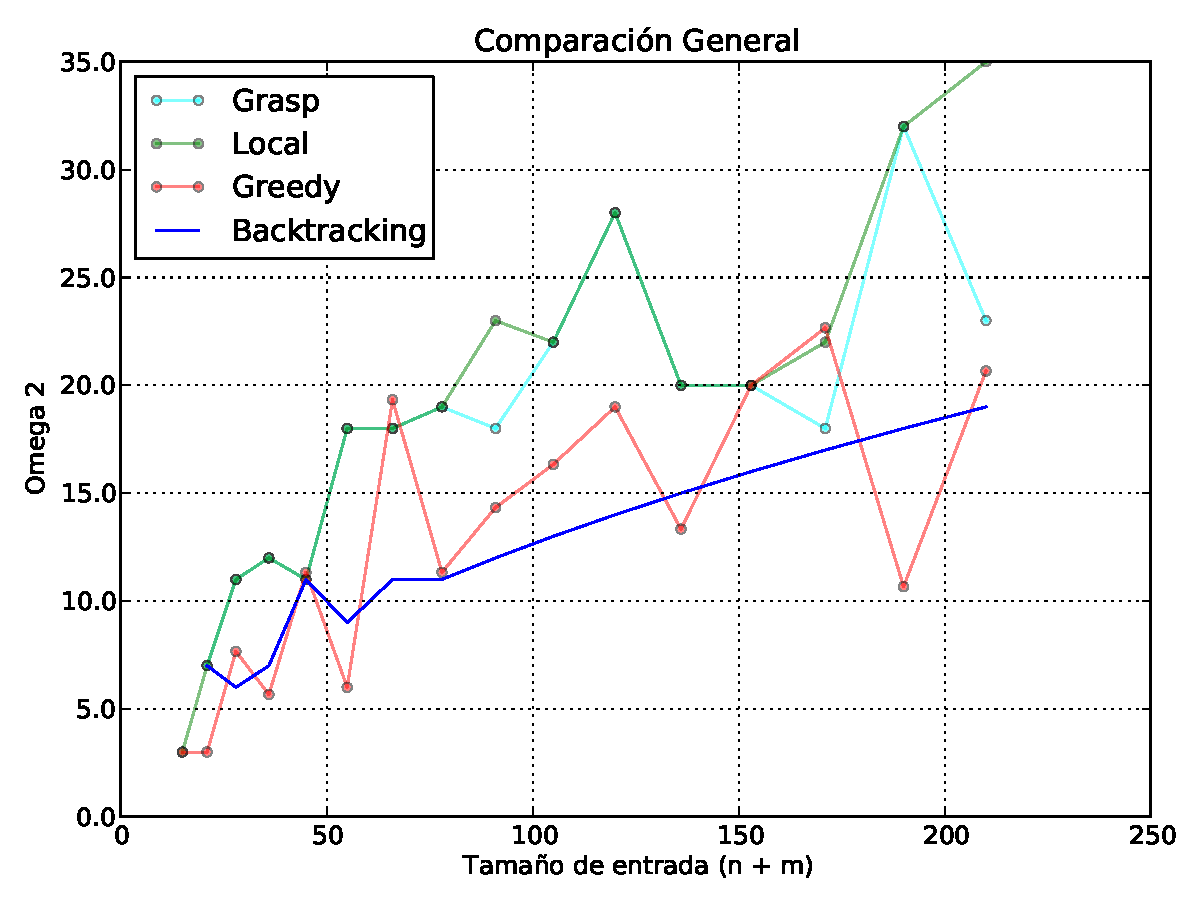
\includegraphics[angle=90]{imagenes/todas_2014-06-27_19-05-53.pdf}
    \label{fig:comparativa}
  \end{figure}

\begin{figure}[H]
\begin{center}
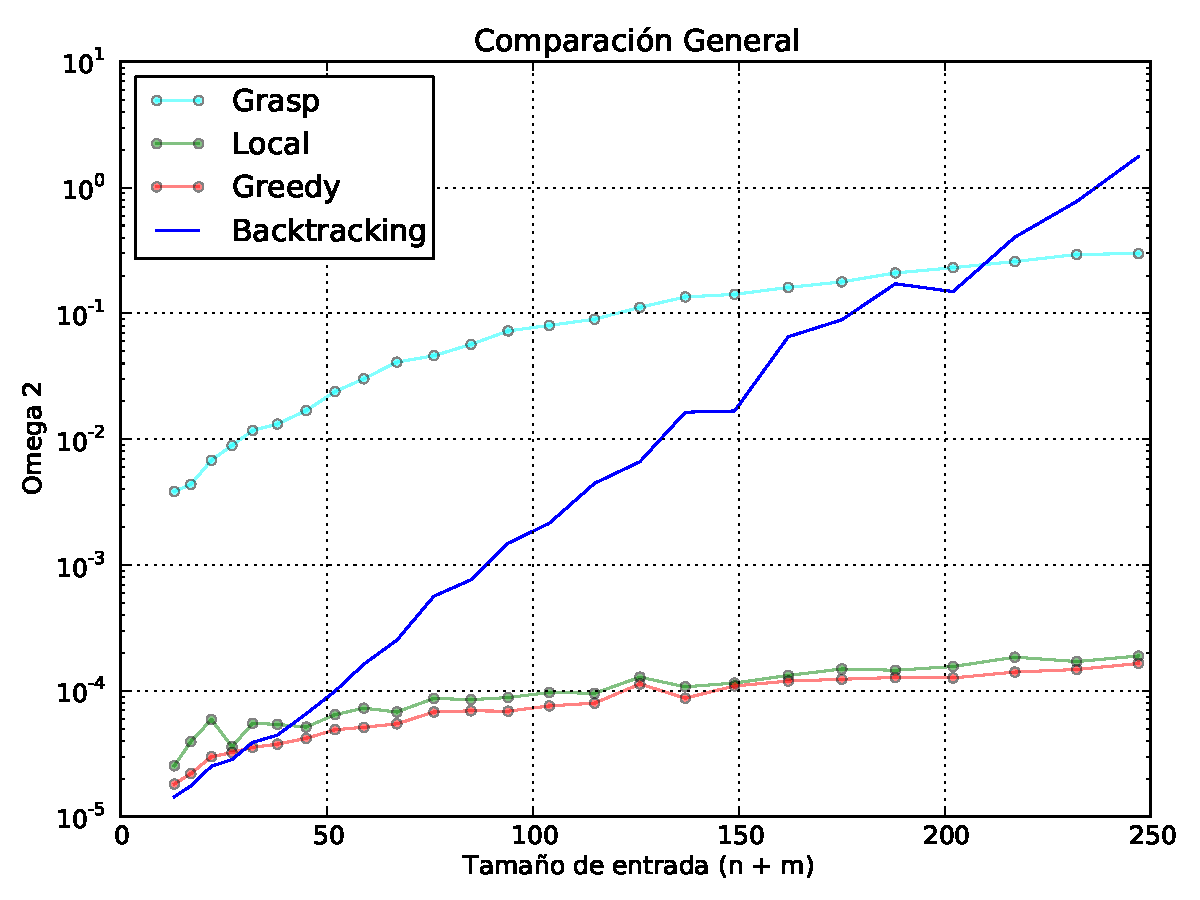
\includegraphics[angle=0, scale=.75]{imagenes/todas-tiempo.pdf}
\label{grafico local}
\end{center}
\end{figure}

\begin{figure}[H]
\begin{center}
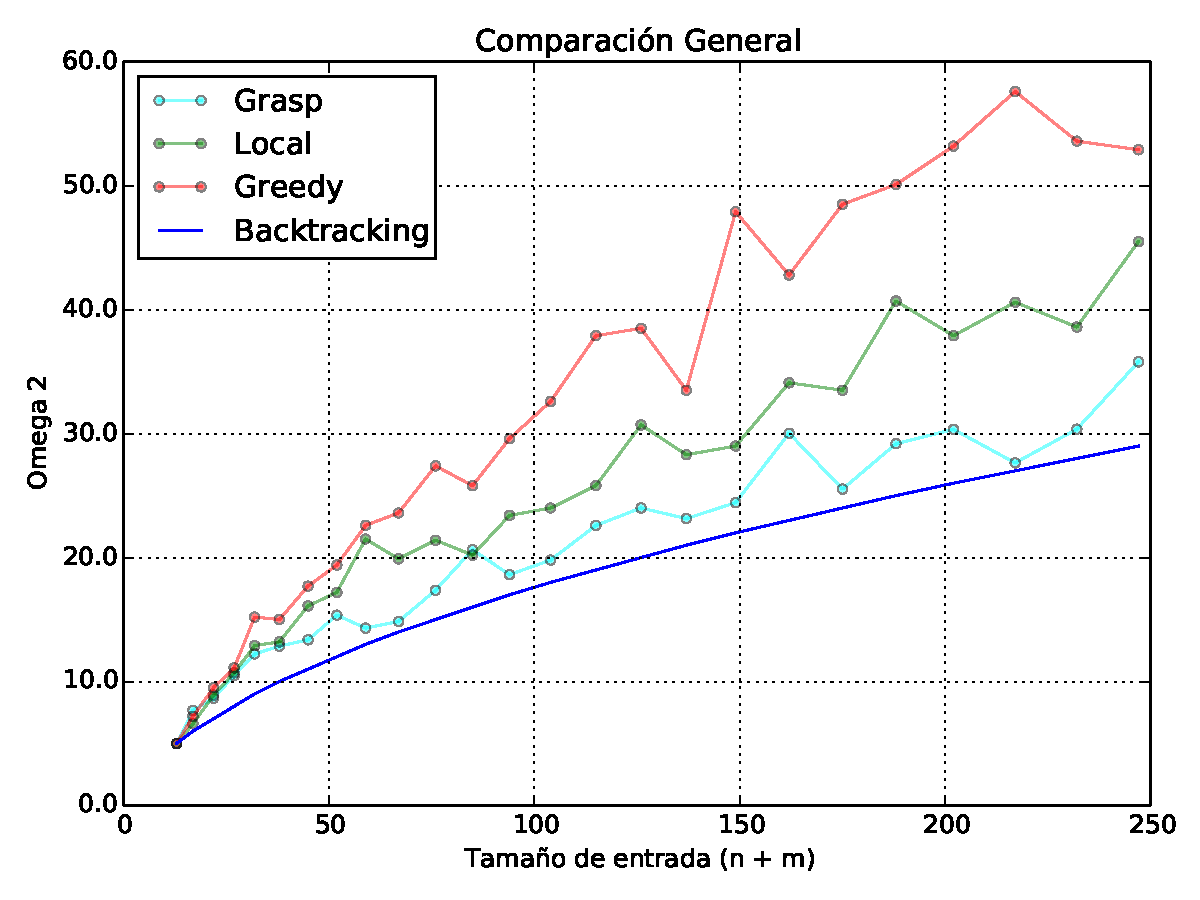
\includegraphics[angle=0, scale=.75]{imagenes/todas-calidad.pdf}
\label{grafico local}
\end{center}
\end{figure}

  Asumimos trivialmente que el backtracking es el algoritmo que logra una mejor \textbf{calidad} al momento de obtener la solución, característica que sólo puede ser contrastada frente al inmenso tiempo que el mismo demora en correr. Resulta también interesante observar el comportamiento del \textbf{algoritmo goloso}, el cual presenta ejecuciones relativamente buenas, mientras que otras ejecuciones directamente no encuentran el algoritmo (se pasan del K); para poder representar este fenómeno se las representó por debajo del algoritmo exacto, de forma tal que se entiende que en las instancias en que el local arrojó un valor menor al backtracking, es porque la solución obtenida no era factible. Por otra parte, el tiempo de esta heurística es mínimo frente a todo el resto de los algoritmos, representando una buena opción para realizar un ``acercamiento rápido'' o ``estimación'' a la solución, ya sea obteniendo una válida o inválida. Aun así, también es necesario destacar que así como muchas de las instancias obtenidas son ``buenas'' desde cierto punto de vista, es notable el hecho de que muchas veces los resultados obtenidos son, aunque factibles, extremadamente malos en relación a la solución exacta. Esto último nos permite inferir que este tipo de heurísticas no nos permiten realizar una estimación ``segura'' sobre la factibilidad o calidad del resultado obtenido, siendo su resultado más bien una especie de ``tiro de ruleta''. Finalmente podemos observar a las heurísticas locales y GRASP, las cuales presentan soluciones en común, dado que GRASP es básicamente una ``aplicación iterativa'' de la local, combinada con un factor de aleatoriedad y ciertos criterios de terminación. Así, el resultado no nos sorprende al mostrarnos lo que de cierta forma ya esperabamos, la heurística de GRASP se comporta siempre ``mejor o igual'' que la local, es decir, existen instancias en que gracias a la aplicación de la aletoriedad en el goloso inicial, y debido a la iteració, se logra una mejoría notable de la calidad de la solución. Por otro lado, aunque GRASP presenta la desventaja de tener un costo tempral mayor a la local, luego de realizar un correcto \textbf{tuneo} de los criterios de finalización logramos establecer una buena relación tiempo/calidad.
